\documentclass[a4]{article}

\usepackage[left=3cm,right=3cm,top=2cm,bottom=2cm]{geometry} 

\usepackage[utf8]{inputenc} 
\usepackage[           spanish % para poder usar el español
                      ,es-tabla % para los captions de las tablas
                       ]{babel}   
\decimalpoint

\usepackage[bookmarks=true,
            bookmarksnumbered=false, % true means bookmarks in 
                                     % left window are numbered
            bookmarksopen=false,     % true means only level 1
                                     % are displayed.
            colorlinks=true,
            linkcolor=blue,
            urlcolor=cyan]{hyperref}
            
\usepackage[T1]{fontenc}
\usepackage{lmodern}

\usepackage{parskip}
\usepackage{xcolor}

\usepackage{multirow}

\usepackage{amsmath,amssymb,amsthm}

\usepackage{caption}

\usepackage{listings}
\lstset
{ %Formatting for code in appendix
  language=C++, % choose the language of the code
  basicstyle=\fontfamily{pcr}\selectfont\footnotesize\color{black},
  keywordstyle=\color{darkorange}\bfseries, % style for keywords
  numbers=left, % where to put the line-numbers
  numberstyle=\tiny, % the size of the fonts that are used for the line-numbers     
  backgroundcolor=\color{white},
  showspaces=false, % show spaces adding particular underscores
  showstringspaces=false, % underline spaces within strings
  showtabs=false, % show tabs within strings adding particular underscores
  tabsize=2, % sets default tabsize to 2 spaces
  captionpos=b, % sets the caption-position to bottom
  breaklines=true, % sets automatic line breaking
  breakatwhitespace=false, 
}

\usepackage{enumerate}% paquete para poder personalizar fácilmente la apariencia de las listas enumerativas

\usepackage{graphicx} % figuras
\usepackage{subfigure} % subfiguras

\definecolor{darkorange}{rgb}{0.94,0.4,0.0}
	
\usepackage{float} % para controlar la situación de los entornos flotantes

\restylefloat{figure}
\restylefloat{table} 

\newcommand{\HRule}{\rule{\linewidth}{0.5mm}}

\author{David Cabezas Berrido\\ Patricia Córdoba Hidalgo\\ Emilio Hoyo Medina\\ Inmaculada Marín Carballo}
\date{\vspace{-5mm}}

\title{\huge Práctica 3: Algoritmos Greedy \HRule\vspace{-4mm}}

%\setcounter{section}{-1}

\begin{document}
\maketitle
\vspace{20mm}
\tableofcontents
\newpage

\section{Introducción}

El problema del viajante de comercio (TSP) consiste en encontrar el
ciclo hamiltoniano de peso mínimo en un grafo conexo y ponderado. En
esta práctica intentaremos abordar este problema por tres algoritmos
greedy distintos.

\subsection{Enfoque greedy}

Primero identificamos las características propias de un problema greedy:
\begin{enumerate}
\item \textbf{Conjunto de candidatos:} Las distintas ciudades a
  recorrer, que serán los nodos del grafo.
\item \textbf{Candidatos ya usados:} Ciudades ya añadidas al ciclo.
\item \textbf{Criterio solución:} Una permutación del conjunto de
  ciudades es solución.
\item \textbf{Criterio factible:} Cualquier lista de ciudades (no
  repetidas) puede llegar a ser solución.
\item \textbf{Función de selección:} A determinar por el algoritmo.
\item \textbf{Función objetivo:} A un ciclo solución le asocia la suma
  de los pesos de las aristas de dicho ciclo (debemos minimizarla).
\end{enumerate}

\section{Algoritmos}

\subsection{Algoritmo del vecino más cercano}

Se toma un vértice cualquiera y se añade al conjunto solución, nosotros
tomamos el primero. A continuación buscamos el vértice más cercano a
éste, y se añade también a la solución. Seguimos tomando el vértice
más cercano al último añadido que no esté en el conjunto
solución y repetimos el proceso hasta que todos los vértices estén en
el conjunto solución.

\subsubsection{Código}

\begin{lstlisting}
  vector<int> result(n);
  result[0] = 0;

  int dmin;
  int sumDistances=0;
  for(int k = 1; k < n; k++){
    dmin = INT_MAX;

    for(j = 0; j < n; j++)
      if(find(result.begin(),result.end(),j) == result.end()){
        distance = map[max(j,result[k-1])][min(j,result[k-1])];
        if(distance < dmin){
          i = j;
          dmin = distance;
        }
      }
      sumDistances += dmin;
      result[k] = i;
    }

  sumDistances += map[max(result[0],result[n-1])][min(result[0],result[n-1])];  
\end{lstlisting}

\subsubsection{Eficiencia teórica}
  
\subsection{Algoritmo de inserción}

Partimos de un recorrido parcial, que incluye la ciudad más al norte,
la ciudad más al este y más al oeste. A continuación, buscamos la
ciudad (entre los candidatos sin escoger) y la posición (en el ciclo)
que supongan un menor incremento en el peso del ciclo y añadimos dicha
ciudad en esa posición. Repetimos este proceso hasta que todos los
vértices estén en el conjunto solución.

\subsubsection{Código}

\begin{lstlisting}
  int sumDistances=0;
  vector<int> result(3);

  //Incluimos las tres ciudades iniciales 
  result[0]=maxX;
  result[1]=minX;
  result[2]=maxY;

  //Sumo las distancias de las 3 ciudades entre ellas
  sumDistances += map[max(result[1],result[0])][min(result[1],result[0])];
  sumDistances += map[max(result[2],result[0])][min(result[2],result[0])];
  sumDistances += map[max(result[1],result[2])][min(result[1],result[2])];

  //Creo un vector con las ciudades que quedan por recorrer (borro las 3 ya escogidas)
  vector<int> candidates(n);
  for(i = 0; i < n; i++) candidates[i]=i;
  candidates.erase(remove(candidates.begin(),candidates.end(),maxX));
  candidates.erase(remove(candidates.begin(),candidates.end(),minX));
  candidates.erase(remove(candidates.begin(),candidates.end(),maxY));
  
  int bestCity;
  int bestPosition;
  int bestD;
  int d;

  while(candidates.size()>0){ // Mientras que queden candidatos (ciudades sin recorrer)
    for(i = 0; i < candidates.size(); i++){
      bestD = INT_MAX;
      for(j = 0; j < result.size(); j++){ // Miro cual es el incrementodel peso que supone insertar esa ciudad en cada posible posicion
        d = map[max(result[j],candidates[i])][min(result[j],candidates[i])]
        + map[max(result[(j+1)%result.size()],candidates[i])]
             [min(result[(j+1)%result.size()],candidates[i])]
        - map[max(result[(j+1)%result.size()],result[j])]
             [min(result[(j+1)%result.size()],result[j])];
        if(d < bestD){ //Buscamos la ciudad y la posicion que minimicen el incremento de la distancia
          bestCity = candidates[i];
          bestPosition = (j+1)%result.size();
          bestD = d;
        }
      }
    }
    result.insert(next(result.begin(),bestPosition),bestCity); //inserto la ciudad en el vector de resultados
    candidates.erase(remove(candidates.begin(),candidates.end(),bestCity)); //borro la ciudad del vector de candidatos
    sumDistances += bestD; //Sumo la distancia a la distancia total del recorrido
  }
\end{lstlisting}

\subsubsection{Eficiencia teórica}

\subsection{Nuestra propuesta: Algoritmo ...} %Ver el de Dijstra

\subsubsection{Código}

\subsubsection{Eficiencia teórica}

\section{Resultados}

A continuación mostramos los ciclos obtenidos por los distintos
algoritmos en una serie de ejemplos y el peso de estos ciclos.

\subsection{ulysses16}

\begin{figure}[H]
  \centering
\subfigure[Ciudades]{\label{graf:ulysses16}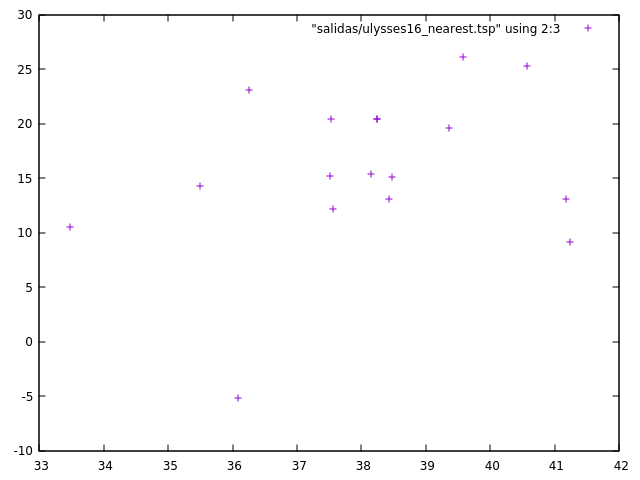
\includegraphics[width=55mm]{graficas/ulysses16}}
\subfigure[Algoritmo de cercanía. Peso = 103]{\label{graf:ulysses16_nearest}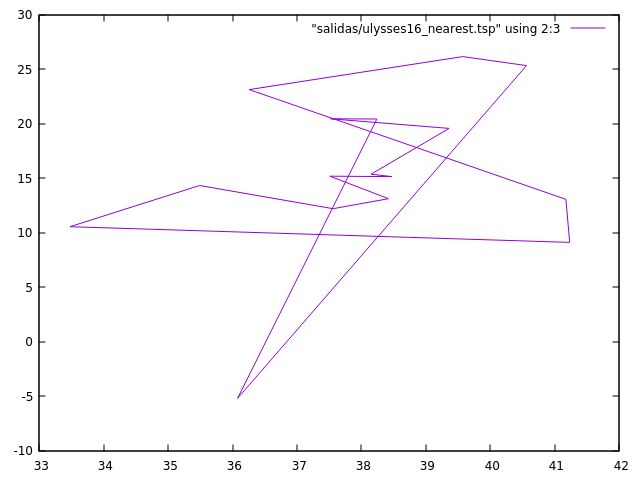
\includegraphics[width=55mm]{graficas/ulysses16_nearest}}
\subfigure[Algoritmo de inserción. Peso = 72]{\label{graf:ulysses16_insertion}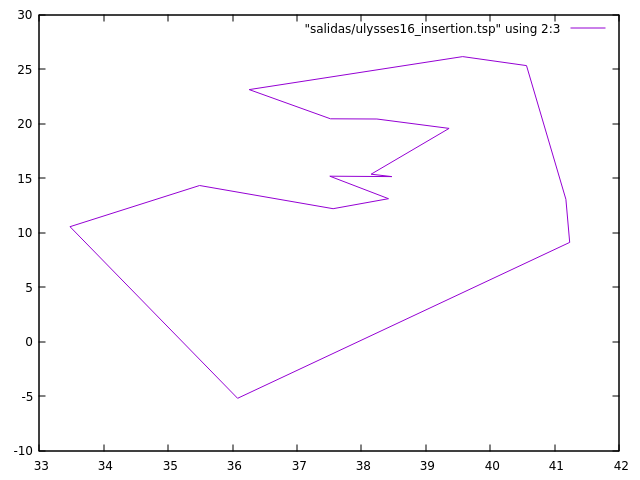
\includegraphics[width=55mm]{graficas/ulysses16_insertion}}
%\subfigure[Algoritmo .... Peso = ]{\label{graf:ulysses16_...}\includegraphics[width=55mm]{graficas/ulysses16_...}}
\end{figure}

\subsection{st70}
\setcounter{subfigure}{0}

\begin{figure}[H]
  \centering
\subfigure[Ciudades]{\label{graf:st70}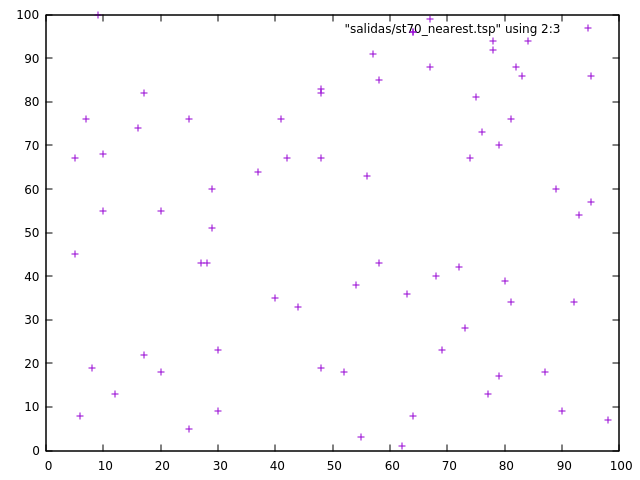
\includegraphics[width=55mm]{graficas/st70}}
\subfigure[Algoritmo de cercanía. Peso = 830]{\label{graf:st70_nearest}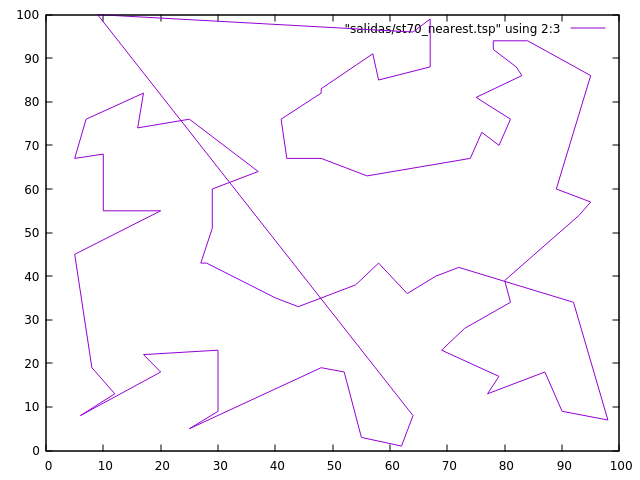
\includegraphics[width=55mm]{graficas/st70_nearest}}
\subfigure[Algoritmo de inserción. Peso = 754]{\label{graf:st70_insertion}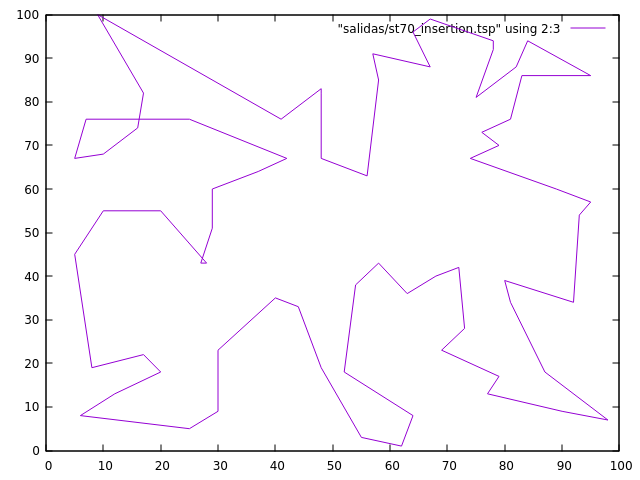
\includegraphics[width=55mm]{graficas/st70_insertion}}
%\subfigure[Algoritmo .... Peso = ]{\label{graf:st70_...}\includegraphics[width=55mm]{graficas/st70_...}}
\end{figure}

\subsection{gr202}
\setcounter{subfigure}{0}

\begin{figure}[H]
  \centering
\subfigure[Ciudades]{\label{graf:gr202}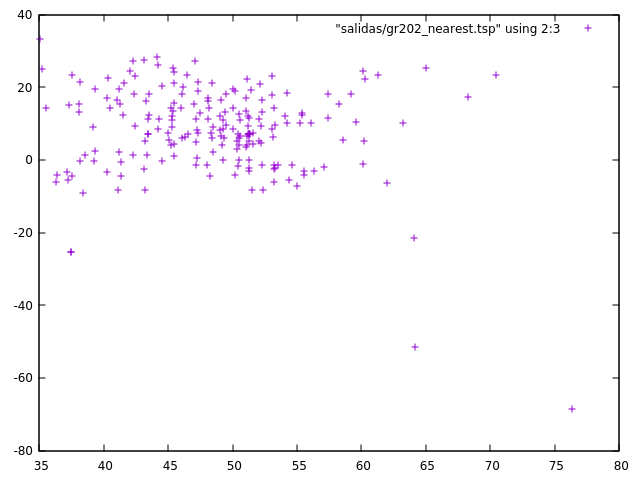
\includegraphics[width=55mm]{graficas/gr202}}
\subfigure[Algoritmo de cercanía. Peso = 651]{\label{graf:gr202_nearest}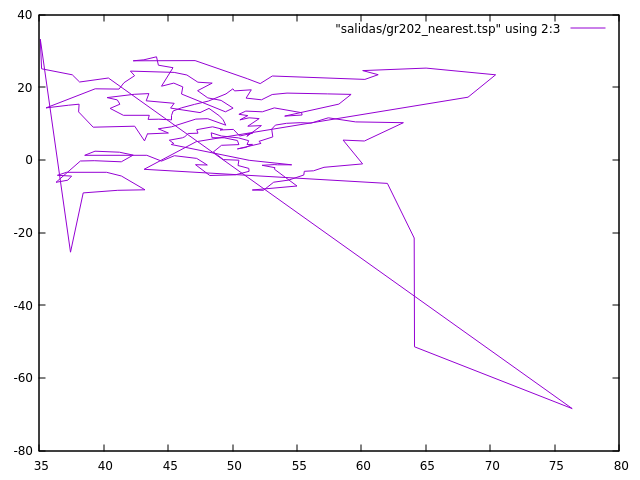
\includegraphics[width=55mm]{graficas/gr202_nearest}}
\subfigure[Algoritmo de inserción. Peso = 554]{\label{graf:gr202_insertion}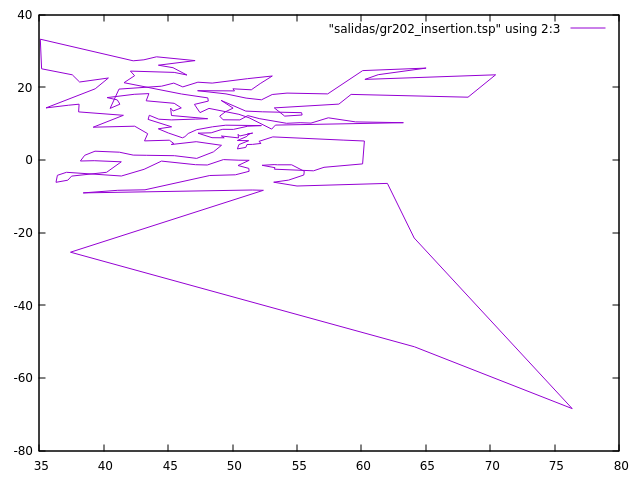
\includegraphics[width=55mm]{graficas/gr202_insertion}}
%\subfigure[Algoritmo .... Peso = ]{\label{graf:gr202_...}\includegraphics[width=55mm]{graficas/gr202_...}}
\end{figure}

\subsection{gr666}
\setcounter{subfigure}{0}

\begin{figure}[H]
  \centering
\subfigure[Ciudades]{\label{graf:gr666}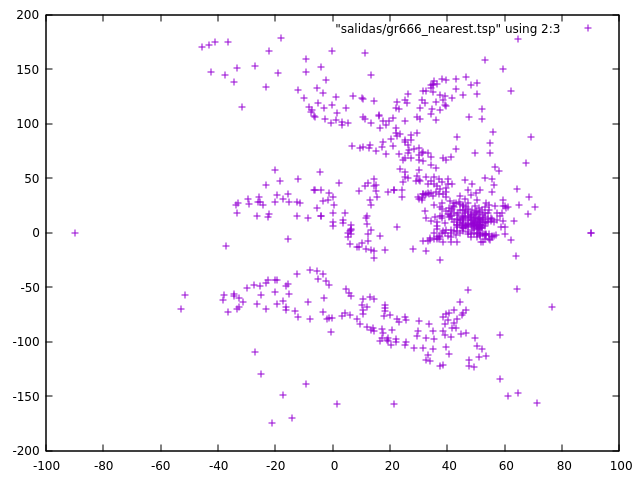
\includegraphics[width=55mm]{graficas/gr666}}
\subfigure[Algoritmo de cercanía. Peso = 4046]{\label{graf:gr666_nearest}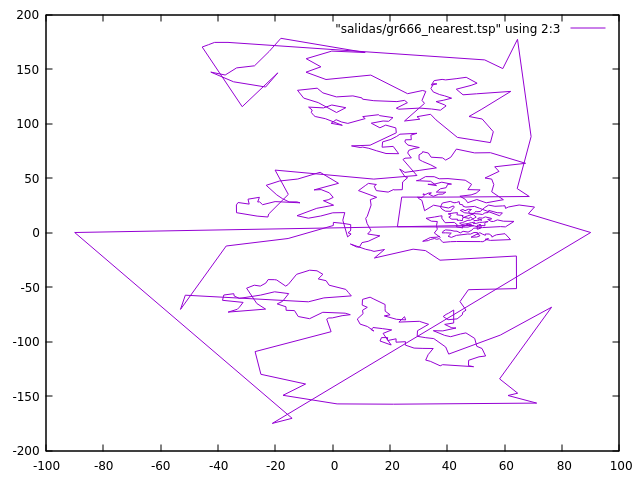
\includegraphics[width=55mm]{graficas/gr666_nearest}}
\subfigure[Algoritmo de inserción. Peso = 3656]{\label{graf:gr666_insertion}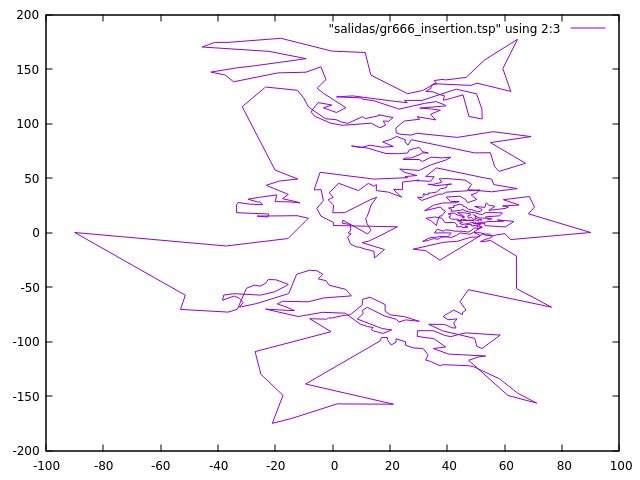
\includegraphics[width=55mm]{graficas/gr666_insertion}}
%\subfigure[Algoritmo .... Peso = ]{\label{graf:gr666_...}\includegraphics[width=55mm]{graficas/gr666_...}}
\end{figure}

\subsection{pr1002}
\setcounter{subfigure}{0}

\begin{figure}[H]
  \centering
\subfigure[Ciudades]{\label{graf:pr1002}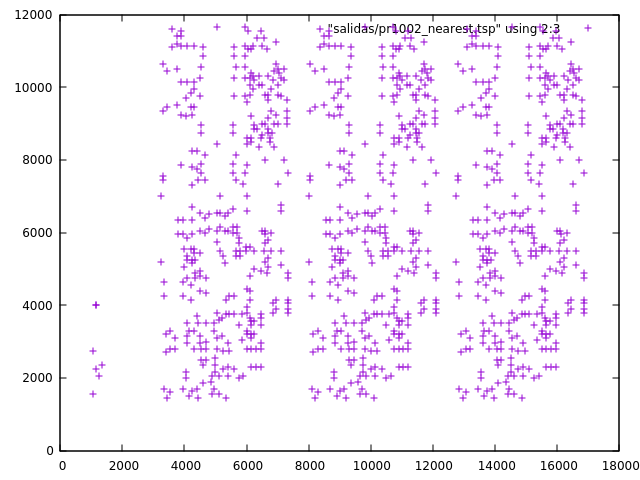
\includegraphics[width=55mm]{graficas/pr1002}}
\subfigure[Algoritmo de cercanía. Peso = 331103]{\label{graf:pr1002_nearest}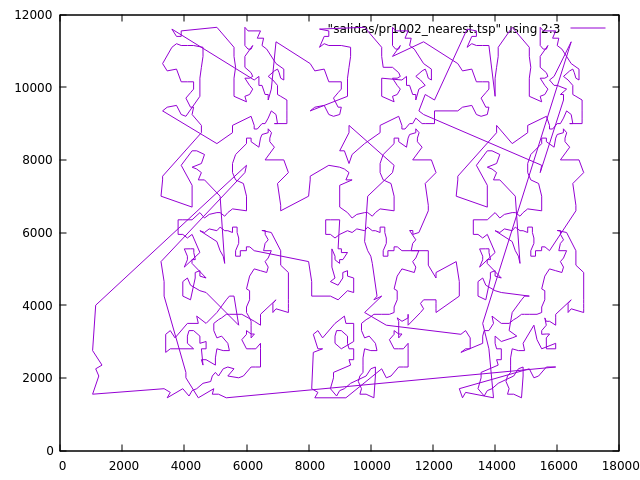
\includegraphics[width=55mm]{graficas/pr1002_nearest}}
\subfigure[Algoritmo de inserción. Peso = 316968]{\label{graf:pr1002_insertion}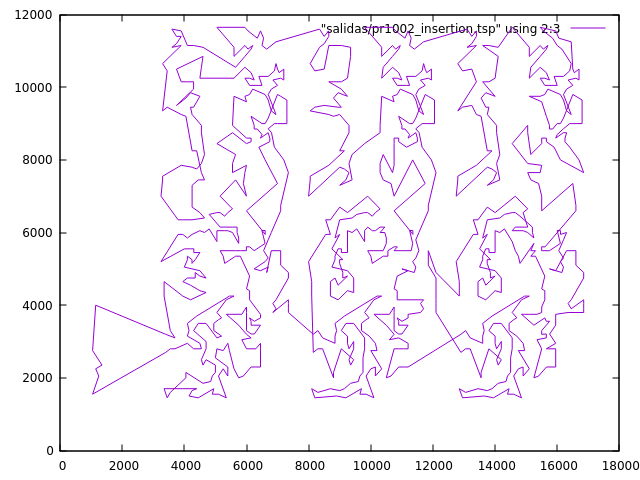
\includegraphics[width=55mm]{graficas/pr1002_insertion}}
%\subfigure[Algoritmo .... Peso = ]{\label{graf:pr1002_...}\includegraphics[width=55mm]{graficas/pr1002_...}}
\end{figure}

\end{document}